\documentclass{article}          % article mode
\usepackage{beamerarticle}

\usepackage[english]{babel}
\usepackage[latin1]{inputenc}
\usepackage{times}
\usepackage[T1]{fontenc}
\usepackage{wordlike}
% \usepackage[text={6.3in,8.2in},centering]{geometry}

\usepackage{amsfonts,amsmath,amssymb,amsthm,mathrsfs,graphicx,subfigure}
\usepackage{bm,ifthen,calc,xspace,hyperref}
% \usepackage{tikz}
% \usetikzlibrary{arrows,positioning,fit,shapes,calc}
\DeclareMathOperator*{\argmin}{\arg\min}
\DeclareMathOperator*{\argmax}{\arg\max}

% Below are knitr-generated code copied from another file.
\usepackage[]{color}
%% maxwidth is the original width if it is less than linewidth
%% otherwise use linewidth (to make sure the graphics do not exceed the margin)
\makeatletter
\def\maxwidth{ %
  \ifdim\Gin@nat@width>\linewidth
    \linewidth
  \else
    \Gin@nat@width
  \fi
}
\makeatother

\definecolor{fgcolor}{rgb}{0.345, 0.345, 0.345}
\newcommand{\hlnum}[1]{\textcolor[rgb]{0.686,0.059,0.569}{#1}}%
\newcommand{\hlstr}[1]{\textcolor[rgb]{0.192,0.494,0.8}{#1}}%
\newcommand{\hlcom}[1]{\textcolor[rgb]{0.678,0.584,0.686}{\textit{#1}}}%
\newcommand{\hlopt}[1]{\textcolor[rgb]{0,0,0}{#1}}%
\newcommand{\hlstd}[1]{\textcolor[rgb]{0.345,0.345,0.345}{#1}}%
\newcommand{\hlkwa}[1]{\textcolor[rgb]{0.161,0.373,0.58}{\textbf{#1}}}%
\newcommand{\hlkwb}[1]{\textcolor[rgb]{0.69,0.353,0.396}{#1}}%
\newcommand{\hlkwc}[1]{\textcolor[rgb]{0.333,0.667,0.333}{#1}}%
\newcommand{\hlkwd}[1]{\textcolor[rgb]{0.737,0.353,0.396}{\textbf{#1}}}%

\usepackage{framed}
\makeatletter
\newenvironment{kframe}{%
 \def\at@end@of@kframe{}%
 \ifinner\ifhmode%
  \def\at@end@of@kframe{\end{minipage}}%
  \begin{minipage}{\columnwidth}%
 \fi\fi%
 \def\FrameCommand##1{\hskip\@totalleftmargin \hskip-\fboxsep
 \colorbox{shadecolor}{##1}\hskip-\fboxsep
     % There is no \\@totalrightmargin, so:
     \hskip-\linewidth \hskip-\@totalleftmargin \hskip\columnwidth}%
 \MakeFramed {\advance\hsize-\width
   \@totalleftmargin\z@ \linewidth\hsize
   \@setminipage}}%
 {\par\unskip\endMakeFramed%
 \at@end@of@kframe}
\makeatother

\definecolor{shadecolor}{rgb}{.97, .97, .97}
\definecolor{messagecolor}{rgb}{0, 0, 0}
\definecolor{warningcolor}{rgb}{1, 0, 1}
\definecolor{errorcolor}{rgb}{1, 0, 0}
\newenvironment{knitrout}{}{} % an empty environment to be redefined in TeX

\usepackage{alltt}
% end knitr related preambles

\begin{document}
% My own macros
\newcommand{\ensuretext}[1]{\ensuremath{\text{#1}}}
\def\ie{\ensuretext{\textit{i.e.,\xspace}}}
\def\eg{\ensuretext{\textit{e.g.,\xspace}}}

\newcommand{\uder}[2]{\frac{\partial #1}{\partial #2}}
\newcommand{\C}{\ensuremath{\mathbb{C}}}
\newcommand{\CP}{\ensuremath{\mathbb{CP}}}
\newcommand{\GL}[1]{\ensuremath{\mathrm{GL}(#1)}}
\newcommand{\SL}[1]{\ensuremath{\mathrm{SL}(#1)}}
\newcommand{\Q}{\ensuremath{\mathbb{Q}}}
\newcommand{\R}{\ensuremath{\mathbb{R}}}
\newcommand{\RP}{\ensuremath{\mathbb{RP}}}
\newcommand{\Z}{\ensuremath{\mathbb{Z}}}
\newcommand{\med}{\ensuremath{\mathop{\mathrm{med}}}}
\newcommand{\uPr}{\ensuremath{\mathop{\mathrm{Pr}}}}
\newcommand{\uE}{\ensuremath{\mathrm{E}}}
\newcommand{\ucov}[2]{\ensuremath{\mathop{\mathrm{cov}}\left(#1 ,\, #2\right)}}
\newcommand{\ucor}[2]{\ensuremath{\mathop{\mathrm{corr}}\left(#1 ,\, #2\right)}}
\newcommand{\ucorr}[2]{\ensuremath{\mathop{\mathrm{corr}}\left(#1 ,\, #2\right)}}
\newcommand{\uvar}{\ensuremath{\mathop{\mathrm{var}}}}
\newcommand{\ud}{\ensuremath{\mathrm{d}}}
\newcommand{\uProj}{\ensuremath{\mathop{\mathrm{Proj}}}}
\newcommand{\uimply}{\ensuremath{\;\Longrightarrow\;}}
\newcommand{\uequiv}{\ensuremath{\;\Longleftrightarrow\;}}
\newcommand{\uforall}{\textrm{ for all }}
\newcommand{\us}[1]{\ensuremath{\mathrm{Sym}(#1)}}
\newcommand{\uo}[2]{\mathrm{Orb}_{#1}(#2)}
\newcommand{\ustab}[1]{\mathrm{Stab}(#1)}
\newcommand{\uinner}[2]{\ensuremath{\langle #1 ,\; #2 \rangle}}
\newcounter{myN}
\newcommand{\urepeat}[2]{%
  \setcounter{myN}{0}
  \whiledo{\value{myN} < #1}{%
    \stepcounter{myN}#2}}
\newcommand{\uvec}[2][n]{\ensuremath{#2_1, \cdots, #2_{#1}}}
\newcommand{\umark}[1]{\marginpar{%
    \vskip-\baselineskip %raise the marginpar a bit
    \raggedright\footnotesize
    \itshape\hrule\smallskip#1\par\smallskip\hrule}}





%%%%%%%%%%%%%% Front matters

\begin{frame}
  \titlepage
\end{frame}

%%%%%%%%%%%%% Main text



\section{Prerequisites}

\begin{frame}
  \frametitle{\texttt{R} and BioConductor}
  \begin{itemize}
  \item \texttt{R} is an advanced statistical programming language and
    data analysis environment. From programming point of view, it
    bears many similarities with \texttt{MATLAB}. 
  \item \texttt{R} is free software.  You can obtain and install it
    from \href{http://www.r-project.org/}.  If you run Linux, I
    recommend you install it from your package management system.
  \item BioConductor is a large collection of \texttt{R} libraries
    designed for analyzing high-throughput genomic data.  
  \end{itemize}
\end{frame}

\begin{frame}[fragile]
  \frametitle{Installing BioConductor}
  Install BioConductor from \texttt{R} is simple
\begin{knitrout}\footnotesize
\definecolor{shadecolor}{rgb}{0.969, 0.969, 0.969}\color{fgcolor}\begin{kframe}
\begin{alltt}
\hlcom{# source("http://bioconductor.org/biocLite.R")}
\hlcom{# biocLite()}
\end{alltt}
\end{kframe}
\end{knitrout}

Once BioConductor is installed, you can install specific package by the same \texttt{biocLite()} function

\begin{knitrout}\footnotesize
\definecolor{shadecolor}{rgb}{0.969, 0.969, 0.969}\color{fgcolor}\begin{kframe}
\begin{alltt}
\hlcom{# biocLite(c("ALL", "genefilter", "GOstats", "samr", "multtest", "GEOquery"))}
\end{alltt}
\end{kframe}
\end{knitrout}

\end{frame}


\section{Welcome to the world of *-omics data!}

\begin{frame}
  \frametitle{Gene expressions}
  \begin{itemize}
  \item The most commonly used bioinformatics data are some form of
    gene expressions, measured by techniques such as microarrays
    (RNA/DNA microarrays, exonarray, beads array, etc) and RNA-seq
    (miRNA-seq, ribosomal profiling, etc).
  \item While microarray and RNA-seq technologies use very different
    approaches, at the end of the day, they both can report expression
    levels as a $m\times n$ dimensional matrix.
  \item Here $m$ is the number of units such as genes or exons, $n$ is
    the number of samples.
  \item Typically $m$ is in the range of $20\sim 50$ thousands, and
    $n$ is in the range of $10\sim 100$. This is a typical ``large
    $p$, small $n$'' scenario in statistical analysis.
  \end{itemize}
\end{frame}

\begin{frame}
  \frametitle{Other *-omics data (I)}
  \begin{itemize}
  \item Though we focus on gene expression data analysis in this talk,
    we would like to point out that many other *-omics data exist.
  \item PCR (Polymerase chain reaction) data. Low throughput
    (cheaper); high sensitivity; often used \emph{after}
    high-throughput gene expression analysis to \emph{confirm}
    differentiation of specific genes.
  \item Protein binding microarray (\textit{a.k.a.} biochip,
    proteinchip).  Records protein instead of DNA/RNA
    expressions. Good for identifying protein-protein interactions;
    transcription factor protein-activation; antibody measurements.
  \end{itemize}
\end{frame}

\begin{frame}
  \frametitle{Microarray Data pre-processing}
  \begin{itemize}
  \item Raw scanner level data on Affymetrix platform are images with
    ``\texttt{.CEL}'' suffixes.  \texttt{R/BioConductor} provides a
    function \texttt{ReadAffy()} to read these CEL files into
    \texttt{R}.
  \item The default preprocessing method provided by
    \texttt{R/BioConductor} is RMA (Robust Multichip Average) which includes
    \begin{enumerate}
    \item Background correction at the image level.
    \item Quantile normalization, which calibrates all arrays to the
      same scale (all quantiles must be the same).
    \item Summarization. Multiple ($15-25$) probes are used to detect
      one target so they need to be summarized to one number.
    \item Variance stabilization transformation.  Most common VST:
      log2 transformation\footnote{Average in the log-scale is
        the \emph{geometric mean}; multiplicative noise becomes
        additive in the log-scale, etc.}.
    \end{enumerate}
  \end{itemize}
\end{frame}

\begin{frame}{RNA-seq data pre-processing}
  \begin{itemize}
  \item Acquire the raw sequence data. For example, on Illumina
    platform, this initial step produces (huge) \texttt{FASTQ} files.
  \item Alignment. In the second step, these raw sequences are aligned
    to a well annotated reference genome.  If one piece of sequence is
    aligned to a known genetic unit (exon, gene, or splice junctions),
    we count one ``match''. Tools: TopHat, BowTie2, etc.  Output file:
    \texttt{BAM} or \texttt{SAM} file.
  \item \texttt{Rsamtools} to work with BAM files; \texttt{Rsubread}
    to turn these files into counting matrix.
  \item Normalization.  Note that once you normalize the counts, most
    tools that are designed specifically for RNA-seq, such as
    \texttt{DESeq2}, no longer apply.  Instead, you should use
    microarray-oriented tools.
  \end{itemize}
\end{frame}


\section{Now we have the data. Which genes are ``interesting''?}

\begin{frame}[fragile]
  \frametitle{Load the ALL data}
  Let us load a sample data (\texttt{ALL}, Acute Lymphoblastic
    Leukemia) first.
\begin{knitrout}\footnotesize
\definecolor{shadecolor}{rgb}{0.969, 0.969, 0.969}\color{fgcolor}\begin{kframe}
\begin{alltt}
\hlcom{## biocLite("ALL")}
\hlkwd{library}\hlstd{(ALL)}      \hlcom{#This is a data library}
\hlkwd{data}\hlstd{(}\hlstr{"ALL"}\hlstd{)}       \hlcom{#a 12,625 by 128 dim matrix }
\hlkwd{print}\hlstd{(ALL)}        \hlcom{#print out some useful information}
\end{alltt}
\end{kframe}
\end{knitrout}
Object: \texttt{ExpressionSet}; features (genes/probesets): 12625; sample size: 128.
\end{frame}

\begin{frame}[fragile,shrink]
  \frametitle{Select a subset of arrays}
  Assume that we want to select only sample from B-cell lymphomas
  harboring the BCR/ABL translocation and from lymphomas with no
  observed cytogenetic abnormalities (NEG).
\begin{knitrout}\footnotesize
\definecolor{shadecolor}{rgb}{0.969, 0.969, 0.969}\color{fgcolor}\begin{kframe}
\begin{alltt}
\hlcom{## BT is the variable of ALL which distinguish B cells}
\hlcom{## from T cells. }
\hlcom{## Show in another window: as.character(ALL[["BT"]])}
\hlstd{bcell} \hlkwb{<-} \hlkwd{grep}\hlstd{(}\hlstr{"^B"}\hlstd{,} \hlkwd{as.character}\hlstd{(ALL[[}\hlstr{"BT"}\hlstd{]]))}

\hlcom{## select molecular types of BCR/ABL and NEG}
\hlstd{molbiol} \hlkwb{<-} \hlkwd{as.character}\hlstd{(ALL[[}\hlstr{"mol.biol"}\hlstd{]])}
\hlstd{moltype} \hlkwb{<-} \hlkwd{which}\hlstd{(molbiol} \hlopt \hlkwd{c}\hlstd{(}\hlstr{"BCR/ABL"}\hlstd{,} \hlstr{"NEG"}\hlstd{))}

\hlstd{data1} \hlkwb{<-} \hlstd{ALL[,} \hlkwd{intersect}\hlstd{(bcell, moltype)]}
\hlcom{## drop unwanted levels of mol.biol}
\hlstd{data1[[}\hlstr{"mol.biol"}\hlstd{]]} \hlkwb{<-} \hlkwd{factor}\hlstd{(data1[[}\hlstr{"mol.biol"}\hlstd{]])}
\end{alltt}
\end{kframe}
\end{knitrout}
 The result, \texttt{data1}, has 79 arrays (42 NEG, 37 BCR/ABL).
\end{frame}

\begin{frame}[fragile]
  \frametitle{Nonspecific filtering}
  \begin{itemize}
  \item Filter out genes \alert{before} statistical analysis.  The
    filtering criteria often include basic quality control
    characteristics such as minimum expression level and standard
    deviation (or interquartile range).
\begin{knitrout}\footnotesize
\definecolor{shadecolor}{rgb}{0.969, 0.969, 0.969}\color{fgcolor}\begin{kframe}
\begin{alltt}
\hlkwd{library}\hlstd{(genefilter)}
\hlcom{## filter based on expression levels}
\hlstd{filter1} \hlkwb{<-} \hlkwd{rowMax}\hlstd{(}\hlkwd{exprs}\hlstd{(data1))}\hlopt{>=}\hlnum{4.0}

\hlcom{## filter based on standard deviation}
\hlstd{filter2} \hlkwb{<-} \hlkwd{rowSds}\hlstd{(}\hlkwd{exprs}\hlstd{(data1))}\hlopt{>=}\hlnum{0.25}
\hlstd{data2} \hlkwb{<-} \hlstd{data1[filter1} \hlopt{&} \hlstd{filter2, ]}
\end{alltt}
\end{kframe}
\end{knitrout}
  \item The result, \texttt{data2}, has 79 arrays and 8411 genes.
  \end{itemize}
\end{frame}


\begin{frame}
  \frametitle{Hypothesis testing} In principle, any parametric or
  nonparametric statistic designed for single hypothesis testing may
  be useful in microarray.  In practice, the following test statistics
  are wided used in microarray data analysis:
  \begin{itemize}
  \item Two sample student $t$-statistic
  \item Wilcoxon rank-sum statistic
  \item Kolmogorov-Smirnov statistic
  \item Cram\'er-von Mises statistic
  \item $N$-statistic
  \end{itemize}
\end{frame}

\begin{frame}
  \frametitle{Two sample student $t$-statistic} 
  \begin{itemize}
  \item Two sample student $t$-statistic is a parametric statistic. In
    order to compute the $p$-value associated with a $t$-statistic
    from the standard $t$-distribution, we need to assume the
    underlying distribution of expression levels are normally
    distributed.
  \item Remark: You can still compute $t$-statistic when data are not
    normally distributed.  But you can not obtain a valid $p$-value by
    looking up the \alert{standard $t$-distribution}.
  \item In fact, a permutation version of $t$-test is valid even for
    non-normal data.
  \end{itemize}
\end{frame}

\begin{frame}
  \frametitle{Two sample student $t$-statistic} 
  \begin{equation}
    \label{eq:t}
    t_{i} = \frac{\bar{\mathbf{x}}^{(A)}_{i}-\bar{\mathbf{x}}^{(B)}_{i}} {\sqrt{s^2_{i}(\frac{1}{n_{A}}+\frac{1}{n_{B}})}}.
  \end{equation}
  where $\bar{\mathbf{x}}^{(A)}_{i}$, $\bar{\mathbf{x}}^{(B)}_{i}$
  represents the mean expressions of the $i$th gene in two phenotypic
  groups ($A$ and $B$); $n_{A}$, $n_{B}$ are the number of arrays of
  each phenotype; $s^{2}_{i}$ is an estimated variance pooled from
  both groups.
\end{frame}

\begin{frame}
  \frametitle{Fold difference, and why it is bad}
  Fold difference\footnote{Fold difference is similar but not
    identical to fold change due to log2 transformation.} is simply
  the difference between $\bar{x}$ and $\bar{y}$.
  \begin{itemize}
  \item[Data 1] $\mathbf{x}^{(A)} = \{1,2,3\}$, $\mathbf{x}^{(B)} = \{4,5,6\}$,
  \item[Data 2] $\mathbf{x}^{(A)} = \{10,20,30\}$, $\mathbf{x}^{(B)} = \{40,50,60\}$.
  \end{itemize}
  Fold differences: 3 for Data 1, 30 for Data 2.  $t$-statistics:
  -3.6742 for both data sets.  $p$-values: 0.02131 for both data sets.
  \cite{Shi2006MicroArrayQualityControl,Klebanov2007Statisticalmethodsand}
\end{frame}

\begin{frame}
  \frametitle{SAM (significant analysis of Microarrays)} A compromise:
  the SAM (significant analysis of Microarrays) approach
  \cite{Tusher2001}.
    \begin{equation}
      \label{eq:sam}
      t_{i,\text{SAM}} = \frac{\bar{\mathbf{x}}^{(A)}_{i}-\bar{\mathbf{x}}^{(B)}_{i}} {\sqrt{(s^2_i + s^{2}_{0})(\frac{1}{n_{A}}+\frac{1}{n_{B}})}}.
    \end{equation}
    where $s^{2}_{0}$ is estimated from the other genes and can be
    considered as a) an estimate of the variance of background noise;
    b) a way to stabilize the signal-to-noise ratio.
\end{frame}

\begin{frame}
  \frametitle{Wilcoxon rank-sum statistic}
  \begin{itemize}
  \item The Wilcoxon rank-sum statistic is a nonparametric alternative
    to $t$-statistic:
    \begin{equation}
      \label{eq:wilcoxon}
      W_{i} = \sum^{n_1}_{j=1} r(x^{(A)}_{ij})
    \end{equation}
  \item Where $r(x^{(A)}_{ij})$ is the rank of $x^{(A)}_{ij}$ in the
    combined sample.
  \item The key point: only ranking information are needed, so
    \begin{enumerate}
    \item $p$-value computed from this statistic is valid even when
      the distribution of the expression levels are not normal.
      \cite{Gibbons1992NonparametricStatisticalInference}
    \item outliers have less effect to inference.
    \end{enumerate}
  \end{itemize}
\end{frame}

\begin{frame}
  \frametitle{Wilcoxon rank-sum statistic} 
  \begin{itemize}
  \item For both Data 1 and Data 2, $W=6$, $p=0.1$. Notice that, this
    $p$-value is greater than the one computed from the $t$-statistic
    (0.02131).
  \item Generally speaking, nonparametric tests are less powerful than
    their parametric counterparts, because we assume that we have some
    \textit{a priori} information about the underlying distribution in
    the parametric case.
  \end{itemize}
\end{frame}

\begin{frame}
  \frametitle{Other advanced statistics} 
  \begin{itemize}
  \item Kolmogorov-Smirnov statistic: a distribution free statistic
    which can be thought of as a \alert{distance} between two
    empirical distribution functions. Its parametric counterpart is
    the $\chi^2$-statistic.
  \item Cram\'er-von Mises statistic: a distribution free statistic
    which was first designed to test the normality of a given
    empirical distribution, it can also be used as a \alert{distance}
    between two empirical distribution functions.
  \item The granularity of this statistic (which causes inaccuracy of
    the corresponding $p$-values) is smaller than that for the
    Kolmogorov-Smirnov statistic, but this statistic and its associate
    $p$-value is much harder to compute.
    \cite{Xiao2007C++ProgramCramer-von}
  \end{itemize}
\end{frame}

\begin{frame}
  \frametitle{Permutation $N$-test} 
  \begin{itemize}
  \item Another nonparametric test based on the $N$-distance between
    two empirical distribution functions.
  \item it is a family of distribution functions depending on the
    \alert{kernel} being used. We can use kernels that are more
    sensitive to a certain kind of departure to get better power.
  \item For instance, by using $L^1$ kernel, this statistic is more
    sensitive to a departure in shifting.
    \cite{Klebanov2005permutationtestmotivated}.
  \item This is also used in differential association studies
    \cite{hu08:_detec_inter_correl_chang_in_microar_analy,rui2009b,Needham2011}.
  \end{itemize}
\end{frame}

\begin{frame}[plain,fragile]
Hypothesis testing (using t-statistics)
\begin{knitrout}\footnotesize
\definecolor{shadecolor}{rgb}{0.969, 0.969, 0.969}\color{fgcolor}\begin{kframe}
\begin{alltt}
\hlstd{tt} \hlkwb{<-} \hlkwd{rowttests}\hlstd{(data2,} \hlstr{"mol.biol"}\hlstd{)}
\end{alltt}
\end{kframe}
\end{knitrout}
Report top 5 differentially expressed probe sets and their gene symbols.
\begin{knitrout}\footnotesize
\definecolor{shadecolor}{rgb}{0.969, 0.969, 0.969}\color{fgcolor}\begin{kframe}
\begin{alltt}
\hlstd{tt.sorted} \hlkwb{<-} \hlstd{tt[}\hlkwd{order}\hlstd{(tt[[}\hlstr{"p.value"}\hlstd{]]), ]}
\hlstd{top5} \hlkwb{<-} \hlkwd{rownames}\hlstd{(tt.sorted)[}\hlnum{1}\hlopt{:}\hlnum{5}\hlstd{]}
\hlkwd{library}\hlstd{(}\hlstr{"hgu95av2.db"}\hlstd{)}
\hlstd{top5.table} \hlkwb{<-} \hlkwd{cbind}\hlstd{(}\hlkwd{links}\hlstd{(hgu95av2SYMBOL[top5]),tt.sorted[}\hlnum{1}\hlopt{:}\hlnum{5}\hlstd{,])}
\hlkwd{print}\hlstd{(}\hlkwd{xtable}\hlstd{(top5.table),} \hlkwc{file}\hlstd{=}\hlstr{"results/table-top5.tex"}\hlstd{)}
\end{alltt}
\end{kframe}
\end{knitrout}
\end{frame}

\begin{frame}
  \frametitle{Top differentially expressed genes}
  % latex table generated in R 3.2.0 by xtable 1.7-3 package
% Fri May 29 15:31:16 2015
\begin{table}[ht]
\centering
\begin{tabular}{rllrrr}
  \hline
 & probe\_id & symbol & statistic & dm & p.value \\ 
  \hline
1 & 1635\_at & ABL1 & 9.26 & 1.10 & 0.00 \\ 
  2 & 1636\_g\_at & ABL1 & 8.69 & 1.15 & 0.00 \\ 
  3 & 1674\_at & YES1 & 7.28 & 1.20 & 0.00 \\ 
  4 & 39730\_at & ABL1 & 6.90 & 1.43 & 0.00 \\ 
  5 & 40504\_at & PON2 & 6.57 & 1.18 & 0.00 \\ 
   \hline
\end{tabular}
\end{table}

\end{frame}


  

\begin{frame}[plain]
  \frametitle{A heatmap of the top 50 DEGs}
  \vspace{-.1in}
    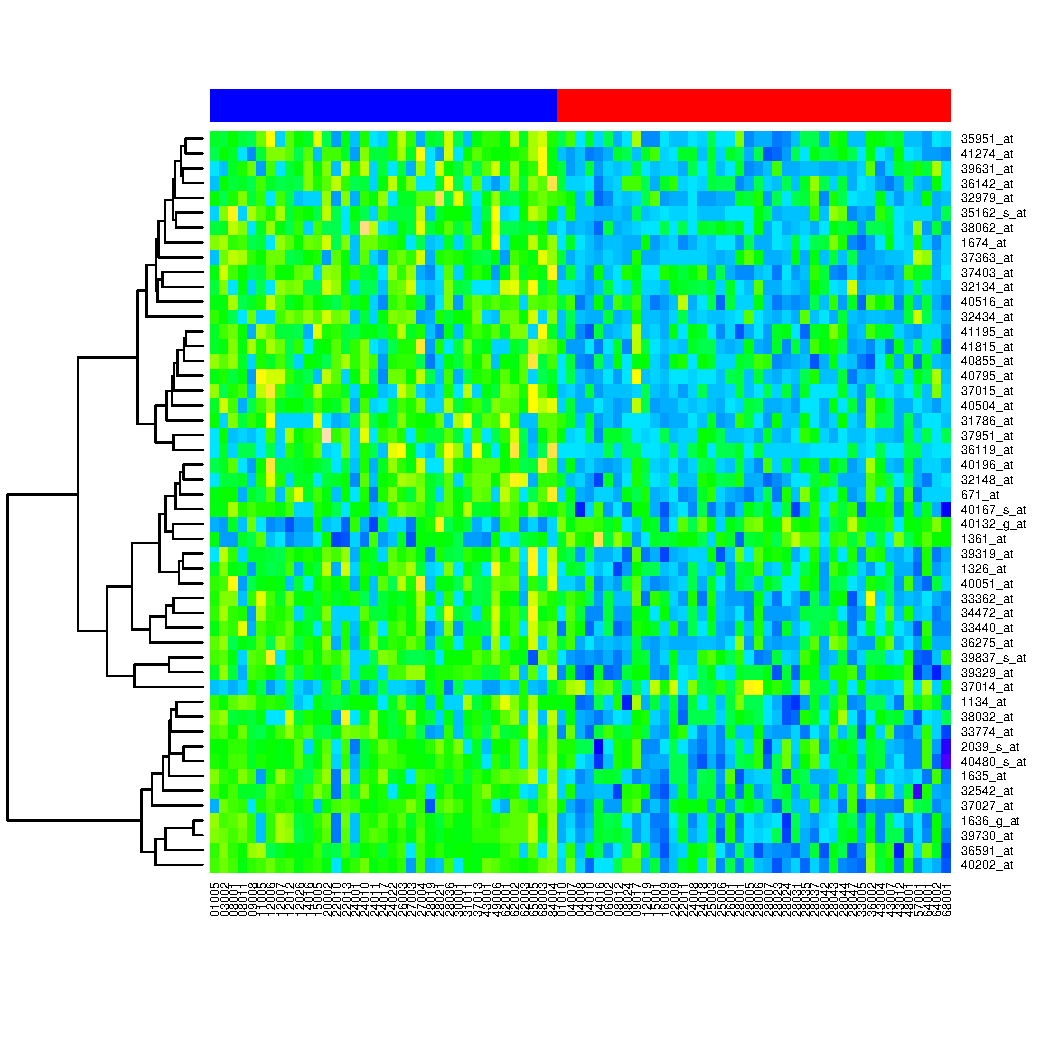
\includegraphics[width=3.8in]{results/heatmap}
\end{frame}

\begin{frame}[fragile]{SAM example}
\begin{knitrout}\footnotesize
\definecolor{shadecolor}{rgb}{0.969, 0.969, 0.969}\color{fgcolor}\begin{kframe}
\begin{alltt}
\hlcom{## The phenotypic information contained in data2}
\hlstd{pheno2} \hlkwb{<-} \hlkwd{pData}\hlstd{(data2)}
\hlcom{## organize the expressions, grouping, genenames, whether}
\hlcom{## data have been log2 transformed into one list.}
\hlstd{input}\hlkwb{=}\hlkwd{list}\hlstd{(}\hlkwc{x}\hlstd{=}\hlkwd{exprs}\hlstd{(data2),} \hlkwc{y}\hlstd{=pheno2[[}\hlstr{"mol.biol"}\hlstd{]],}
    \hlkwc{geneid}\hlstd{=}\hlkwd{as.character}\hlstd{(}\hlnum{1}\hlopt{:}\hlkwd{nrow}\hlstd{(data2)),}
    \hlkwc{genenames}\hlstd{=}\hlkwd{paste}\hlstd{(}\hlstr{"g"}\hlstd{,}\hlkwd{as.character}\hlstd{(}\hlnum{1}\hlopt{:}\hlkwd{nrow}\hlstd{(data2)),}\hlkwc{sep}\hlstd{=}\hlstr{""}\hlstd{),}
    \hlkwc{logged2}\hlstd{=}\hlnum{TRUE}\hlstd{)}
\hlcom{## Please use 1000 permutations in a real application}
\hlstd{samr.obj} \hlkwb{<-} \hlkwd{samr}\hlstd{(input,} \hlkwc{resp.type}\hlstd{=}\hlstr{"Two class unpaired"}\hlstd{,} \hlkwc{nperms}\hlstd{=}\hlnum{100}\hlstd{)}
\hlcom{## detect significant genes}
\hlstd{delta.table} \hlkwb{<-} \hlkwd{samr.compute.delta.table}\hlstd{(samr.obj,}
                   \hlkwc{min.foldchange}\hlstd{=}\hlnum{0.1}\hlstd{,} \hlkwc{nvals}\hlstd{=}\hlnum{200}\hlstd{)}
\hlstd{siggenes.table} \hlkwb{<-} \hlkwd{samr.compute.siggenes.table}\hlstd{(samr.obj,}
                 \hlkwc{del}\hlstd{=}\hlnum{0}\hlstd{, input, delta.table,} \hlkwc{all.genes}\hlstd{=}\hlnum{TRUE}\hlstd{)}
\hlkwd{sum}\hlstd{(}\hlkwd{as.numeric}\hlstd{(siggenes.table}\hlopt{$}\hlstd{genes.up[,} \hlstr{"q-value(%)"}\hlstd{])}\hlopt{<}\hlnum{5}\hlstd{)}
\hlkwd{sum}\hlstd{(}\hlkwd{as.numeric}\hlstd{(siggenes.table}\hlopt{$}\hlstd{genes.lo[,} \hlstr{"q-value(%)"}\hlstd{])}\hlopt{<}\hlnum{5}\hlstd{)}
\end{alltt}
\end{kframe}
\end{knitrout}
  
\end{frame}

\begin{frame}[fragile]{RNA-seq data, SAM}
  
\begin{knitrout}\footnotesize
\definecolor{shadecolor}{rgb}{0.969, 0.969, 0.969}\color{fgcolor}\begin{kframe}
\begin{alltt}
\hlcom{## please load pasilla.Rdata from the net-drive}
\hlkwd{load}\hlstd{(}\hlstr{"pasilla.Rdata"}\hlstd{)}
\hlkwd{head}\hlstd{(pasillaExp)}
\hlstd{pasillaPheno}
\hlcom{### Note that we don't need logged2=TRUE}
\hlstd{input}\hlkwb{=}\hlkwd{list}\hlstd{(}\hlkwc{x}\hlstd{=pasillaExp,} \hlkwc{y}\hlstd{=pasillaPheno,}
    \hlkwc{geneid}\hlstd{=}\hlkwd{as.character}\hlstd{(}\hlnum{1}\hlopt{:}\hlkwd{nrow}\hlstd{(pasillaExp)),}
    \hlkwc{genenames}\hlstd{=}\hlkwd{rownames}\hlstd{(pasillaExp))}
\hlcom{## Notice the assay.type arguement}
\hlstd{samr.obj}\hlkwb{<-}\hlkwd{samr}\hlstd{(input,}  \hlkwc{resp.type}\hlstd{=}\hlstr{"Two class unpaired"}\hlstd{,}
               \hlkwc{assay.type}\hlstd{=}\hlstr{"seq"}\hlstd{,} \hlkwc{nperms}\hlstd{=}\hlnum{100}\hlstd{)}
\hlstd{delta.table} \hlkwb{<-} \hlkwd{samr.compute.delta.table}\hlstd{(samr.obj)}
\hlstd{siggenes.table}\hlkwb{<-}\hlkwd{samr.compute.siggenes.table}\hlstd{(samr.obj,} \hlkwc{del}\hlstd{=}\hlnum{0}\hlstd{, input, delta.table)}
\end{alltt}
\end{kframe}
\end{knitrout}
  
\end{frame}

\begin{frame}[fragile]{RNA-seq, DESeq2}

\begin{knitrout}\footnotesize
\definecolor{shadecolor}{rgb}{0.969, 0.969, 0.969}\color{fgcolor}\begin{kframe}
\begin{alltt}
\hlcom{# object construction}
\hlstd{dds} \hlkwb{<-} \hlkwd{DESeqDataSetFromMatrix}\hlstd{(pasillaExp,} \hlkwd{DataFrame}\hlstd{(pasillaPheno),} \hlopt{~} \hlstd{pasillaPheno)}
\hlcom{# standard analysis}
\hlstd{dds} \hlkwb{<-} \hlkwd{DESeq}\hlstd{(dds)}
\hlstd{res} \hlkwb{<-} \hlkwd{results}\hlstd{(dds)}
\hlkwd{head}\hlstd{(res)}
\hlkwd{sum}\hlstd{(res[,} \hlstr{"padj"}\hlstd{]}\hlopt{<}\hlnum{0.05}\hlstd{,} \hlkwc{na.rm}\hlstd{=}\hlnum{TRUE}\hlstd{)}
\end{alltt}
\end{kframe}
\end{knitrout}
  
\end{frame}

\section{How to control false discoveries for 20,000 comparisons}

\begin{frame}
  \frametitle{Type I, II error, testing power}
  \begin{tabular}{|l|c|c|}
    & Accept $H_0$ & Reject $H_0$ \\
    \hline
    $H_0$  & True Negative & False Positive, type I error) \\
    \hline
    $H_1$  & False Negative, type II error & True Positive) \\
  \end{tabular}
\end{frame}
\begin{frame}
  \frametitle{Per-Comparison Error Rate (PCER)} Per-comparison error
  rate, or PCER is the probability of making the type I error in a
  single test. \\
  Under most common scenario, this is precisely determined by the
  threshold of $p$-value to reject $H_0$ (the significance level of the
  test).
\end{frame}

\subsection{Family-wise Error Rate}
\begin{frame}
  \frametitle{Definition of FWER} From now on we assume that we have
  $m$ hypotheses (whether a given gene is diff. exp. or not) to be
  tested simultaneously. By definition, FWER is the probability of
  producing one or more false positives
  \begin{equation}
    \label{eq:fwer}
    FWER = Pr(FP \geq 1)
  \end{equation}
\end{frame}
\begin{frame}
  \frametitle{Why controlling FWER is important} 
  \begin{itemize}
  \item controlling FWER at a significance level $\alpha$ gives us
    $1-\alpha$ confidence to say
    that there is no mistake in the outcome.
  \item Suppose you have done $t$-test for 20,000 genes. At
    significance level $\alpha = 0.05$, how many genes will be
    identified as DEG \alert{by chance}?
  \end{itemize}
\end{frame}

\begin{frame}
  \frametitle{Bonferroni adjustment} Bonferroni adjusted $p$-value:
  $p^{bon}_i = \min (m \times p_i, 1)$ For example, suppose raw
  $p$-value is $0.0428$ and $m=20$, then the Bonferroni adjusted
  $p$-value is $0.856$. A statistical test based on the Bonferroni
  adjusted $p$-values rather than the unadjusted $p$-values is called
  the Bonferroni procedure.
\end{frame}

\begin{frame}
  \frametitle{Relationship to PFER} A related quantity is the
  per-family error rate (PFER), the expected number of false
  positives.
  \begin{equation}
    \label{eq:pfer}
    PFER = E(FP)
  \end{equation}
  PFER is always greater or equal to FWER. So any procedure (including
  Bonferroni) which controls PFER controls FWER.  
\end{frame}

\begin{frame}
  \frametitle{Sidak, Holm, etc} Some other less conservative FWER controlling
  procedures exist. These procedures usually adjust $p$-values
  stepwisely, i.e., they order the $p$-values first, then adjust $p_i$
  one by one according to the rank of $p_i$. They may further divided
  into step-down procedures and step-up procedures.
\end{frame}

\begin{frame}
  \frametitle{Correlation and FWER} 
  \begin{itemize}
  \item If we know the relationship of the hypotheses, we may be able
    to utilize this information to get a better procedure (that is,
    more powerful procedure which controls the same nominal FWER
    level).
  \item Westfall and Young procedure uses permutation to generate the
    null distribution. Thus keeps the correlation structure of
    hypotheses. It is time consuming but more powerful than
    Bonferroni.  See
    \cite{Westfall1993Resampling-BasedMultipleTesting}.
  \end{itemize}
\end{frame}

% \begin{frame}
%   \frametitle{Trivial case, Ind. vs. 1.0 correlated} Let us assume
%   $m=20$. If all hypotheses are independent, then on average $1.0$
%   false discovery is expected if the significance level is $0.05$ and
%   we do not apply any MTA. \\
%   What if all hypotheses are correlated with coefficient $1.0$?\\
%   It doen't change the expected number of false discovery, but it does
%   change the probability of having one or more false discovery.
% \end{frame}

\begin{frame}[fragile]
  \frametitle{Bonferroni}
  Bonferroni is simple but conservative.
\begin{knitrout}\footnotesize
\definecolor{shadecolor}{rgb}{0.969, 0.969, 0.969}\color{fgcolor}\begin{kframe}
\begin{alltt}
\hlstd{pvals} \hlkwb{<-} \hlstd{tt[[}\hlstr{"p.value"}\hlstd{]]}
\hlstd{pvals.bonf} \hlkwb{<-} \hlkwd{p.adjust}\hlstd{(pvals,} \hlstr{"bonferroni"}\hlstd{)}
\hlkwd{sum}\hlstd{(pvals.bonf}\hlopt{<}\hlnum{0.05}\hlstd{)}
\end{alltt}
\begin{verbatim}
## [1] 26
\end{verbatim}
\end{kframe}
\end{knitrout}
It finds 26 DEGs.
\end{frame}

\begin{frame}[fragile]
  \frametitle{Westfall and Young}
  Westfall and Young permutation test is a more powerful alternative
\begin{knitrout}\footnotesize
\definecolor{shadecolor}{rgb}{0.969, 0.969, 0.969}\color{fgcolor}\begin{kframe}
\begin{alltt}
\hlkwd{library}\hlstd{(multtest)}
\hlstd{cl} \hlkwb{<-} \hlstd{data1[[}\hlstr{"mol.biol"}\hlstd{]]}\hlopt{==}\hlstr{"NEG"} \hlcom{#class labels}
\hlstd{rr} \hlkwb{<-} \hlkwd{mt.maxT}\hlstd{(}\hlkwd{exprs}\hlstd{(data2), cl,} \hlkwc{B}\hlstd{=}\hlnum{1000}\hlstd{)}

\hlcom{## to get back to the original ordering}
\hlstd{ord} \hlkwb{<-} \hlkwd{order}\hlstd{(rr}\hlopt{$}\hlstd{index)}

\hlcom{## W-Y adjusted p-values}
\hlstd{pvals.wy} \hlkwb{<-} \hlstd{rr}\hlopt{$}\hlstd{adjp[ord]}
\hlkwd{sum}\hlstd{(pvals.wy}\hlopt{<}\hlnum{0.05}\hlstd{)}
\end{alltt}
\end{kframe}
\end{knitrout}
It finds 31 DEGs.
\end{frame}


\subsection{False Discovery Rate}
\begin{frame}
  \frametitle{Definition of the False Discovery Rate (FDR)} the False
  Discovery Rate (FDR) is defined as (roughly) the expected value of
  the ratio of the false positives among all positives.
  \begin{equation}
    \label{eq:fdr}
    FDR = E(Q)
  \end{equation}
  Where $Q=\frac{FP}{FP+TP}$ when there is at least one positive, or
  zero otherwise (to avoid $0/0$).
\end{frame}
\begin{frame}
  \frametitle{Example} Suppose we have $m$ hypotheses to be
  tested. The associated $p$-value for gene $i$ is denoted as
  $p_i$. Then a test designed to control FDR at level $0.05$
  guarantees that out of $20$ discoveries, only one or less is a false
  discovery on average.
\end{frame}
\begin{frame}
  \frametitle{FDR v. FWER/FCER} Like PFER, FDR is an \alert{expected
    number}. While both FWER and FCER based procedures controls
  certain \alert{probability} and fit well with the traditional
  significance testing framework, FDR controlling procedures controls
  an expected value that has a very different statistical meaning.
\end{frame}
\begin{frame}
  \frametitle{Instability of FDR} FDR is the expectation of a
  ratio. When we expect the denominator (total discoveries) to be
  small, small variation in the numerator/denominator can result in
  huge variation of the quotient.
\end{frame}

\begin{frame}[fragile]
  \frametitle{False discovery rate (example)}
Using the Benjamini-Hochberg procedure to control FDR.
\begin{knitrout}\footnotesize
\definecolor{shadecolor}{rgb}{0.969, 0.969, 0.969}\color{fgcolor}\begin{kframe}
\begin{alltt}
\hlstd{pvals.fdr} \hlkwb{<-} \hlkwd{p.adjust}\hlstd{(pvals,} \hlstr{"BH"}\hlstd{)}
\hlkwd{sum}\hlstd{(pvals.fdr}\hlopt{<}\hlnum{0.05}\hlstd{)}
\end{alltt}
\begin{verbatim}
## [1] 199
\end{verbatim}
\end{kframe}
\end{knitrout}
It finds 199 DEGs.
\end{frame}

\section{Machine learning techniques}

\begin{frame}
  \frametitle{Discriminant analysis (supervised machine learning)}
  \begin{itemize}
  \item Select a manageable set of features.  Usually done by
    statistical significant test.
  \item Standardize these features to the same scale.
  \item Split the data into two sets, one (larger) for training and
    one (smaller) for testing.
  \item Train a discriminant function on the training set, and then
    apply the formula to the testing set.
  \item Repeat for many times.
  \end{itemize}
\end{frame}

\begin{frame}
  \frametitle{Linear discriminant analysis}
  \begin{itemize}
  \item The simplest approach is linear discriminant analysis. 
  \item Underline assumptions:
    \begin{enumerate}
    \item the expressions of DEGs follow two multivariate normal
      distributions with the in different phenotypic groups.
    \item covariance structures are the same in these phenotypic groups.
    \item mean expressions are different
    \end{enumerate}
    \begin{equation}
      \label{eq:lda-model}
      \mathbf{x}^{(A)} \sim MVN\left(\bm{\mu}^{(A)},\, \Sigma\right), \quad \mathbf{x}^{(B)} \sim MVN\left(\bm{\mu}^{(B)},\, \Sigma\right).
    \end{equation}
  \item Under these assumptions, the best data driven method to
    separate these two distributions is a hyperplane (a linear
    subspace).
  \end{itemize}
\end{frame}

\begin{frame}[plain,fragile]
  \frametitle{Linear discriminant analysis example}
\begin{knitrout}\footnotesize
\definecolor{shadecolor}{rgb}{0.969, 0.969, 0.969}\color{fgcolor}\begin{kframe}
\begin{alltt}
\hlcom{## The correlations between the 1st, 2nd, and 3rd top DEGs }
\hlcom{## are too high. So I use the 1st and 4th genes for }
\hlcom{## better visualization}

\hlstd{top2} \hlkwb{<-} \hlkwd{t}\hlstd{(}\hlkwd{exprs}\hlstd{(top50set)[}\hlkwd{c}\hlstd{(}\hlnum{1}\hlstd{,}\hlnum{4}\hlstd{),])}
\hlstd{rr.lda} \hlkwb{<-} \hlkwd{lda}\hlstd{(top2, top50set[[}\hlstr{"mol.biol"}\hlstd{]])}
\end{alltt}
\end{kframe}
\end{knitrout}
\end{frame}




\begin{frame}[plain]
  \begin{columns}
  \begin{column}{0.5\textwidth}
    % latex table generated in R 2.15.0 by xtable 1.7-0 package
% Wed Apr 18 15:05:23 2012
\begin{table}[ht]
\begin{center}
\begin{tabular}{rrr}
  \hline
 & BCR/ABL & NEG \\ 
  \hline
BCR/ABL &  29 &   8 \\ 
  NEG &   3 &  39 \\ 
   \hline
\end{tabular}
\caption{Results of linear discriminant analysis. Cross-validation is used for evaluate true/false predictions.}
\label{tab:lda}
\end{center}
\end{table}

  \end{column}

  \begin{column}{0.5\textwidth}
    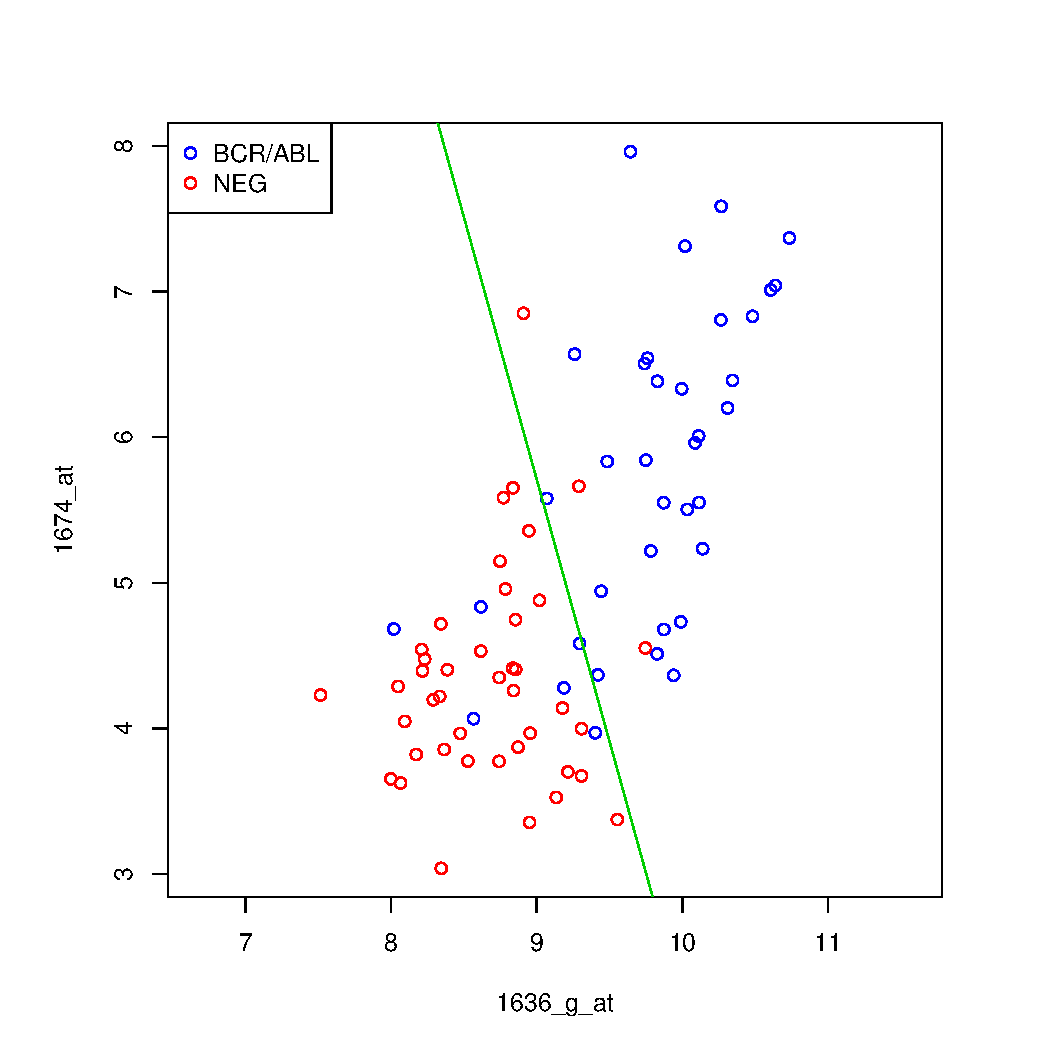
\includegraphics[width=2.5in]{results/lda}
  \end{column}
\end{columns}
\end{frame}


\begin{frame}
  \frametitle{Logistic Regression}
  \begin{itemize}
  \item Alternatively we can use multiple logistic regression
    analysis.
  \item Logistic regression is an example of \emph{generalized linear
      regression}.
  \item For more information you can check out the \texttt{glm()}
    function in \texttt{R}.
  \end{itemize}
\end{frame}

\begin{frame}
  \frametitle{Nonlinear discriminant analysis}
  \begin{itemize}
  \item For \alert{nonlinear} discriminant analysis, support vector
    machine (SVN) and $K$-nearest neighbor methods are the most
    popular choices.
  \item They are implemented in packages \texttt{svn} and \texttt{MLinterfaces}.
  \item Another alternative is random forest, but it has a tendency to
    \textit{overfit} a continuous model.
  \end{itemize}
\end{frame}


\begin{frame}
  \frametitle{Principal component analysis (unsupervised learning)}
  \begin{itemize}
  \item Genes are known to form functionally related sets, which means
    they could be highly correlated.
  \item PCA uses an orthogonal transformation to convert correlated
    gene expressions into a set of \alert{uncorrelated} variables
    called principal components.
  \item Since PCs are uncorrelated, we can divide the total variance
    into variance components explained by each PC.
  \item Empirical evidence shows that just a few PCs can explain 95\%
    of total variance.
  \item Geometrically speaking, this means the observations fit a low
    dimensional hyperplane very well.
  \end{itemize}
\end{frame}

\begin{frame}[plain,fragile]
  \begin{columns}
  \begin{column}{0.5\textwidth}
To compute the principal components are easy
\begin{knitrout}\footnotesize
\definecolor{shadecolor}{rgb}{0.969, 0.969, 0.969}\color{fgcolor}\begin{kframe}
\begin{alltt}
\hlstd{rr.pca} \hlkwb{<-} \hlkwd{prcomp}\hlstd{(top2)}
\end{alltt}
\end{kframe}
\end{knitrout}
The explained standard deviation (shown as the length of vectors):  1.291 (first PC); 0.508 (second PC).
  \end{column}

  \begin{column}{0.5\textwidth}
    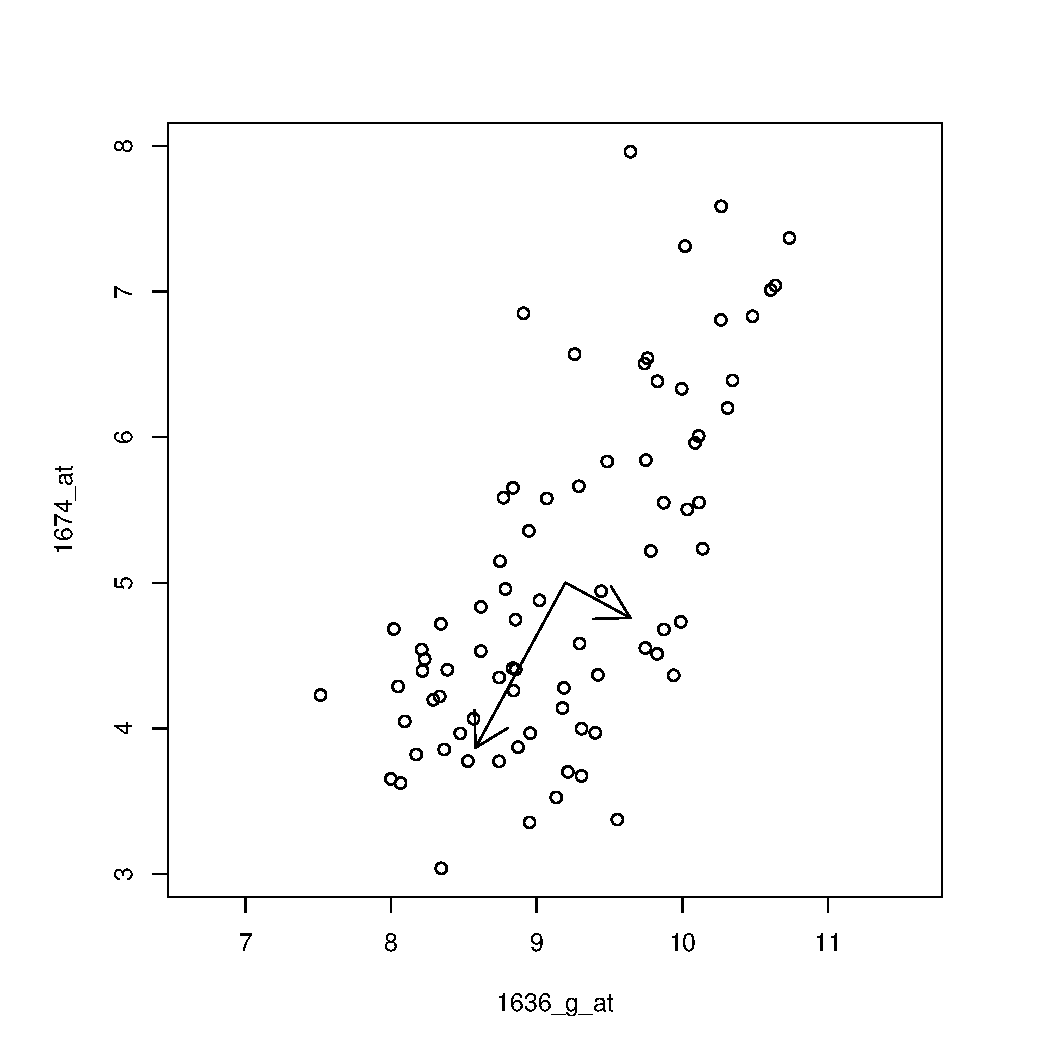
\includegraphics[width=2.5in]{results/pca}
  \end{column}
\end{columns}
\end{frame}




\begin{frame}
  \frametitle{Cluster analysis (unsupervised learning)}
  \begin{itemize}
  \item Feature selection. You can use the top $M$ genes based on
    $p$-value, or the first few principal components computed from all
    significant genes.  The bottom line: no more than 10 features
    otherwise you run the risk of overwhelming the cluster algorithms.
  \item Feature standardization.
  \item Distance/similarity measure. $K$-means uses the Euclidean
    distance. $SK$-means uses spherical distance.
  \item Determine how many clusters.  AIC/BIC
  \item Run the actual cluster analysis. 
  \end{itemize}
\end{frame}

\begin{frame}[plain,fragile]
\begin{knitrout}\footnotesize
\definecolor{shadecolor}{rgb}{0.969, 0.969, 0.969}\color{fgcolor}\begin{kframe}
\begin{alltt}
\hlcom{## compute PCs}
\hlstd{pcs} \hlkwb{<-} \hlkwd{prcomp}\hlstd{(}\hlkwd{t}\hlstd{(}\hlkwd{exprs}\hlstd{(top50set)))}

\hlcom{## take only the first 2 PCs as features}
\hlstd{pc2} \hlkwb{<-} \hlstd{pcs[[}\hlstr{"rotation"}\hlstd{]][,} \hlnum{1}\hlopt{:}\hlnum{2}\hlstd{]}

\hlcom{## feature standardization}
\hlstd{pc2b} \hlkwb{<-} \hlkwd{scale}\hlstd{(pc2)}

\hlcom{## $K$-means clustering}
\hlstd{rr.kmeans} \hlkwb{<-} \hlkwd{kmeans}\hlstd{(pc2b,} \hlnum{2}\hlstd{)}
\end{alltt}
\end{kframe}
\end{knitrout}

\begin{knitrout}\footnotesize
\definecolor{shadecolor}{rgb}{0.969, 0.969, 0.969}\color{fgcolor}\begin{kframe}
\begin{alltt}
\hlcom{## Mclust() is a model based clustering method.}
\hlstd{rr.mclust} \hlkwb{<-} \hlkwd{Mclust}\hlstd{(pc2b)}
\end{alltt}
\end{kframe}
\end{knitrout}
\end{frame}



\begin{frame}[plain,fragile]
  \begin{columns}
  \begin{column}{0.5\textwidth}
    \begin{figure}
      \centering
      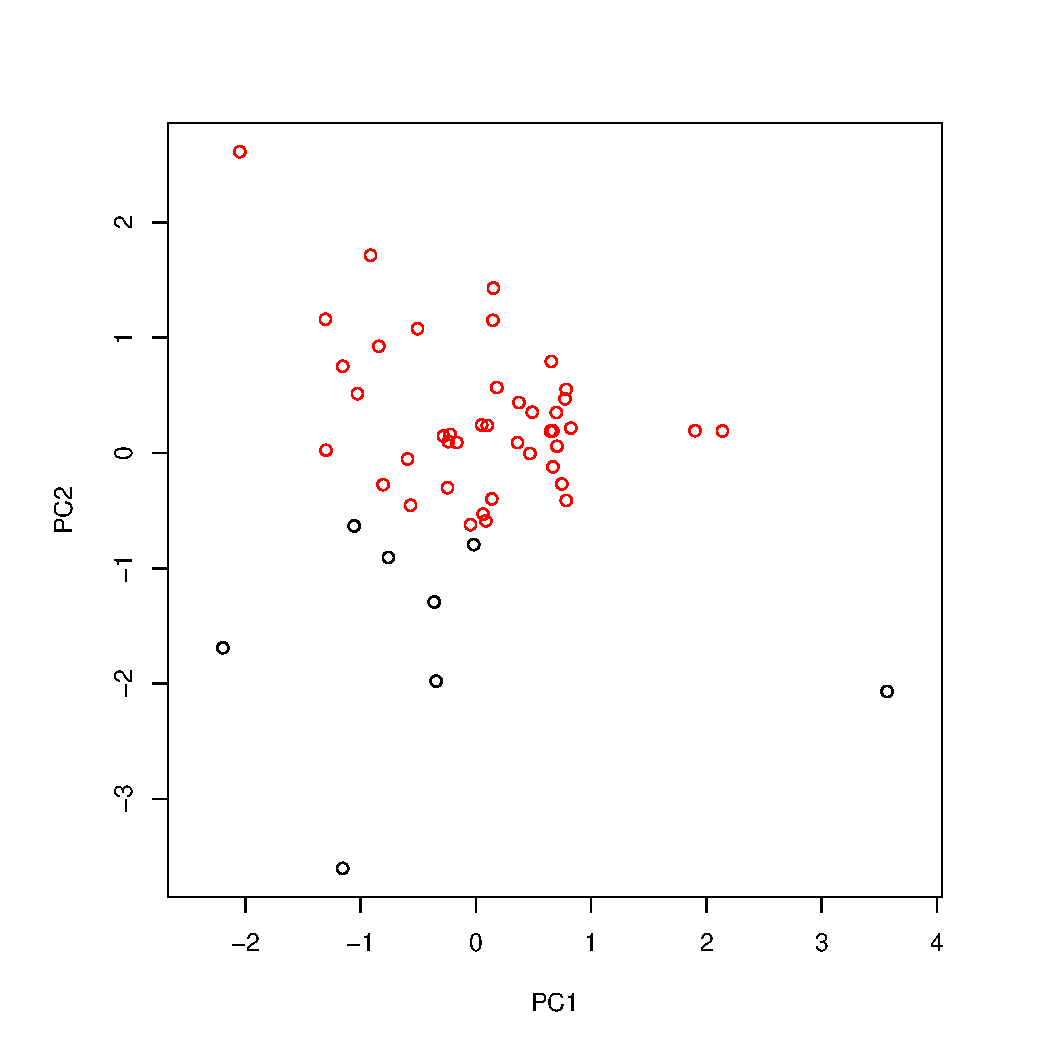
\includegraphics[width=2.5in]{results/kmeans}
      \caption{$K$-means clustering}
      \label{fig:kmeans}
    \end{figure}
  \end{column}

  \begin{column}{0.5\textwidth}
    \begin{figure}
      \centering
      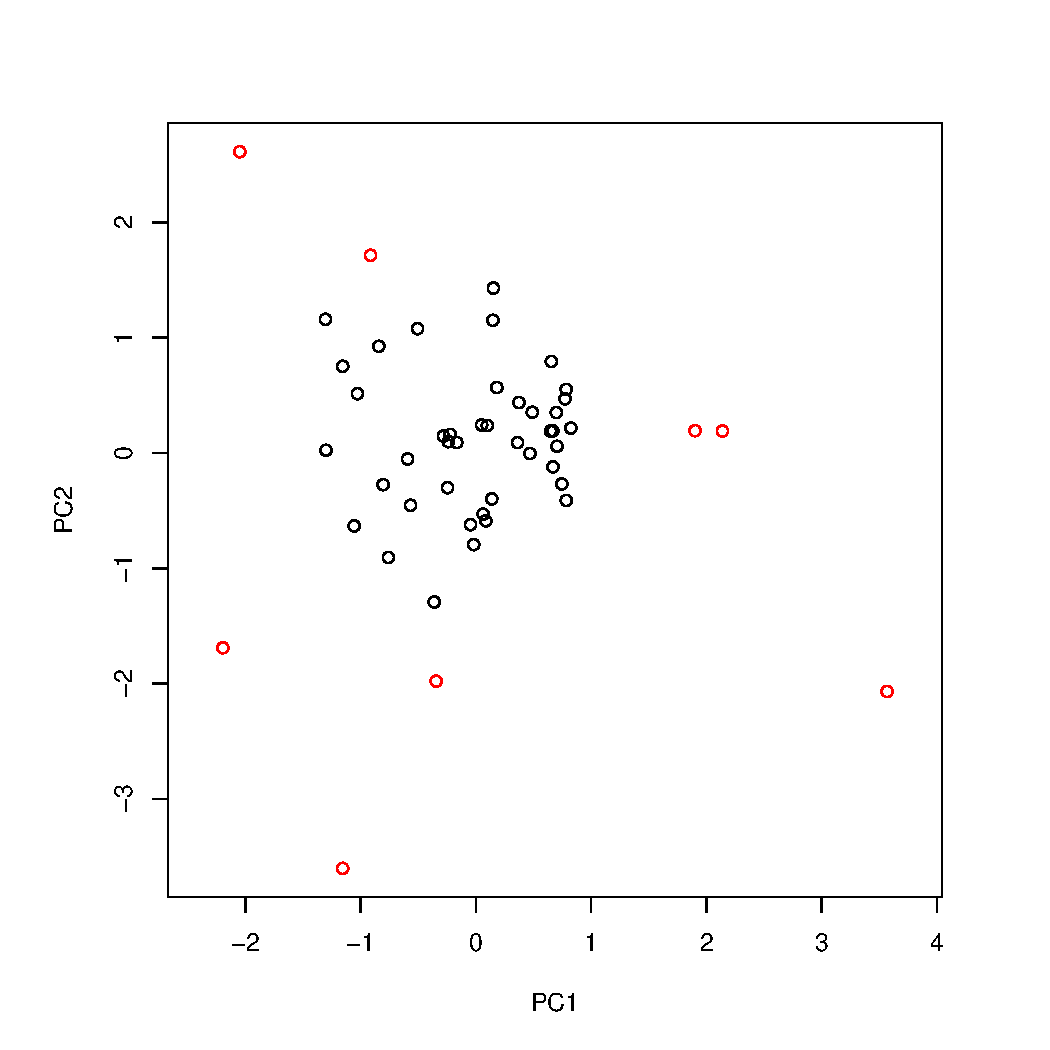
\includegraphics[width=2.5in]{results/mclust}
      \caption{Mclust clustering}
      \label{fig:mclust}
    \end{figure}
  \end{column}
\end{columns}
\end{frame}

\section{Beyond analyzing probe sets}

\begin{frame}
  \frametitle{Gene annotation (I)}
  Gene annotation is tricky because
  \begin{itemize}
  \item Once significant probe sets are identified, we need to map
    them to the corresponding genes and obtain useful information
    about these genes.
  \item This mapping is nontrivial because
    \begin{enumerate}
    \item Multiple probe sets per gene.
    \item Organism level information are grouped in different (and
      numerous) libraries.
    \item Platform dependency.
    \end{enumerate}
  \end{itemize}
\end{frame}

\begin{frame}
  \frametitle{Gene annotation (II)}
  \begin{itemize}
  \item Probe set IDs (\texttt{sig.probes <- rownames(top50set)} or
    \texttt{sig.probes <- featureNames(top50set)}).
  \item Entrez IDs: \texttt{links(hgu95av2ENTREZID[sig.probes])}.
  \item Unigene IDs: \texttt{links(hgu95av2UNIGENE[sig.probes])}.
  \item Gene Symbols: \texttt{links(hgu95av2SYMBOL[sig.probes])}.
  \item GO IDs: \texttt{links(hgu95av2GO[sig.probes])}.
  \item KEGG pathway IDs: \texttt{links(hgu95av2PATH[sig.probes])}.
  \item Chromosome start and stop locs: \textbf{CHRLOC} and
    \textbf{CHRLOCEND}.
  \end{itemize}
\end{frame}

\begin{frame}
  \frametitle{Functional Enrichment Analysis}
  \begin{itemize}
  \item Genes are grouped into sets, such as biological pathways or GO terms.
  \item The rationale of the hypergeometric test.
  \item The implementation. See the next slide.
  \end{itemize}
\end{frame}

\begin{frame}[plain,fragile]{Enrichment analysis example}
\begin{knitrout}\footnotesize
\definecolor{shadecolor}{rgb}{0.969, 0.969, 0.969}\color{fgcolor}\begin{kframe}
\begin{alltt}
\hlcom{## sig.probes are the significant probe sets}
\hlkwd{library}\hlstd{(GOstats)}
\hlstd{sig.probes} \hlkwb{<-} \hlkwd{rownames}\hlstd{(tt)[pvals.fdr}\hlopt{<}\hlnum{0.1}\hlstd{]}
\hlstd{id.table} \hlkwb{<-} \hlkwd{links}\hlstd{(hgu95av2ENTREZID[sig.probes])}
\hlstd{sig.ids} \hlkwb{<-} \hlkwd{unique}\hlstd{(id.table[,}\hlstr{"gene_id"}\hlstd{])}

\hlcom{## entrezUniverse is the set of all (DEGs and NDEGs)}
\hlcom{## probe sets.}
\hlstd{entrezUniverse} \hlkwb{<-} \hlkwd{unlist}\hlstd{(}\hlkwd{mget}\hlstd{(}\hlkwd{rownames}\hlstd{(tt),}
                              \hlstd{hgu95av2ENTREZID))}

\hlstd{params} \hlkwb{<-} \hlkwd{new}\hlstd{(}\hlstr{"GOHyperGParams"}\hlstd{,} \hlkwc{geneIds}\hlstd{=sig.ids,}
              \hlkwc{universeGeneIds}\hlstd{=entrezUniverse,}
              \hlkwc{annotation}\hlstd{=}\hlstr{"hgu95av2.db"}\hlstd{,}
              \hlkwc{ontology}\hlstd{=}\hlstr{"BP"}\hlstd{,}
              \hlkwc{pvalueCutoff}\hlstd{=}\hlnum{0.001}\hlstd{,}
              \hlkwc{conditional}\hlstd{=}\hlnum{FALSE}\hlstd{,}
              \hlkwc{testDirection}\hlstd{=}\hlstr{"over"}\hlstd{)}
\end{alltt}
\end{kframe}
\end{knitrout}
\end{frame}


\begin{frame}[plain,fragile]
\begin{knitrout}\footnotesize
\definecolor{shadecolor}{rgb}{0.969, 0.969, 0.969}\color{fgcolor}\begin{kframe}
\begin{alltt}
\hlcom{## Run the hyper-geometric test for significance.}
\hlstd{rr.gsea} \hlkwb{<-} \hlkwd{hyperGTest}\hlstd{(params)}

\hlcom{## Run a reasonable multiple testing procedure}
\hlstd{pp.gsea} \hlkwb{<-} \hlkwd{pvalues}\hlstd{(rr.gsea)}
\hlstd{pp.gsea.bh} \hlkwb{<-} \hlkwd{p.adjust}\hlstd{(pp.gsea,} \hlstr{"BH"}\hlstd{)}

\hlcom{## Output a table as report.}
\hlstd{nn} \hlkwb{<-} \hlkwd{sum}\hlstd{(pp.gsea.bh}\hlopt{<}\hlnum{0.05}\hlstd{)}
\hlstd{tab.gsea} \hlkwb{<-} \hlkwd{summary}\hlstd{(rr.gsea,}\hlkwc{pvalue}\hlstd{=pp.gsea[nn}\hlopt{+}\hlnum{1}\hlstd{])}
\hlkwd{write.csv}\hlstd{(tab.gsea,} \hlkwc{file}\hlstd{=}\hlstr{"results/table-gsea.csv"}\hlstd{)}
\end{alltt}
\end{kframe}
\end{knitrout}
63 pathways are significant. Show the \texttt{table-gsea.csv} file.
\end{frame}


\begin{frame}
  \frametitle{Other advanced techniques}
  \begin{itemize}
  \item Gene set enrichment analysis. Its relationship to enrichment
    analyses based on discrete tests such as hypergeometric
    test. Package: \texttt{limma}, function \texttt{camera()}.
  \item Network reconstruction. Bayesian network; boolean network.
  \item The use of ODE in network analysis for time-course data.
  \item Differential association analysis.
  \end{itemize}
\end{frame}

\begin{frame}[allowframebreaks]{Bibliography}
  \bibliographystyle{amsplain}
  \bibliography{xing}
\end{frame}




\end{document}
